\chapter{Discussion}
\label{chap:discussion}
Along previous lines we have identified points that need to be discussed regarding our choices and the way this \acrshort{poc} was engineered. This chapter will discuss these points to shed light on the pitfalls of our approach and potential points of improvements or further analysis that could drive the project forward. We won't extensively discuss each point but rather list some ideas.

\section{How Can We Use the Predictions?}
This question should have been solved prior to the project in order to set identifiable goals regarding the prediction algorithm. We collected some ideas regarding the potential way these predictions could be used.

When discussing with the team in charge of designing the support flows that are used by the \acrshort{thd} agent, we discovered that most internet problems are solved without the real need for an agent (e.g. performing cabling checks, rebooting the \acrshort{cpe}, ...). 

Also the call center is open from 8am to 10pm. We need to create the vectors for the past days in order to predict on the current day. Therefore the dataset can be generated from midnight to 1am. 

Some of the fix can be applied remotely. Nevertheless, as we noted previously, failing \acrshort{cpe}s are more likely to be offline and therefore unreachable remotely. It is for this reason that we would propose the following steps:
\begin{enumerate}
	\item \textbf{Tentative remote fix}: upon detecting a failing \acrshort{cpe} overnight, and for those that are reachable the company could try to apply the different remote fixes to the \acrshort{cpe}s (e.g. reboot, update the firmware). Even if the prediction is wrong, during the night these fixes would go unnoticed by the customer. 
	\item \textbf{Self-Care}: notify the customer that a potential problem has been identified with his/her \acrshort{cpe}. Explain the remote steps that have been performed (if they have). Propose the same flow as the one used by the \acrshort{thd} agent in a customer focused manner (vulgarised) to take him/her through the different steps that could solve the problem for example through a smartphone app. 
	\item \textbf{Shortcut}: only in the case where the customer couldn't fix his problem propose a reference that could be used to call the service center and save time to the expert by skipping all the checks that the customer performed on his own. In such case, the experts indicated that most probably the customer would need a swap or a truck roll.
\end{enumerate}

With such approach UPC could improve customer satisfaction by showing its pro-activity, but also it would save time to customers that wouldn't have to wait on the phone to perform basic checks. Finally, it would also reduce the workload put on the call center by restricting interaction with customers to the mere minimum and only in cases where it is necessary. 

\section{Improving Data}
\label{sec:improving}
We have put together a quick business explanation of why we think that the data used by the model for now prevents business from leveraging entirely the value from their data management processes.

\subsection{Recall vs. Precision}
In order to check a prediction with an expert from the \acrshort{hfc} support team, UPC would pay CHF8.54 for the workforce, while servicing a call costs CHF9 in terms of employee salary. These numbers estimated from employee salaries and average handling time show that a strategy of increasing the recall by dropping the precision would not be particularly successful. Indeed it costs approximately the same to service a call and to check a prediction which, moreover, won't fix the problem but simply identify it. 

\subsection{Building the Ground Truth Labelling}
We have highlighted on many occasions the limitations of using \acrshort{via} as our only means to label vectors. First of all, we are discarding many cases out of the analysis for now. Out of the almost 3,000 calls received by UPC for technical help every day, this analysis considers approximately 112 \acrshort{cpe}s every day as sick. On top of which the model can identify approximately 13\% at 90\% precision, 25\% at 80\% precision and 32\% at 70\% accuracy (cf table~\ref{model_comparison}).

A good start would be to change the way that data from the call center is collected to provide more reliable information. The \acrshort{mac} of the \acrshort{cpe} that is being serviced isn't stored for now. It would be easy to collect it and would be a "quick win" to enrich the data. Also rather than using the \acrshort{ftr} flag to decide whether the problem was fixed or not, customer feedback could be used. This would require the help of multiple stakeholders to adapt the servicing process but wouldn't require deep changes and therefore should be implemented without too much difficulty.

New sources of data could also be exploited. As any computer, a \acrshort{cpe} collects software logs that identify potential problems. These logs could be leveraged in order to detect failing \acrshort{cpe}s. We believe that these could be much more precise than using the correlation found between health measurements from the network and \acrshort{cpe} failures. Moreover, these logs could be used to also diagnose \acrshort{cpe}s with a deep sleep mode as we wouldn't need to access them every hour but could set up \acrshort{cpe}s to transmit these logs every day at a given time (exiting deep sleep shortly for such purpose).

Also new sources of data could be leveraged and used to diagnose other flows of problems than internet ones. 

Finally, once predictions are being used, we could leverage customer feedback in order to enrich our labelling and correct potential mistakes. 

\vspace{\baselineskip}
The launch of an internal initiative around artificial intelligence could push different experts in the company to share their knowledge of UPC's assets. But also it would allow potential modification of internal processes to support the development of such solutions.


\section{Improving the Model}
This proof of concept was conducted in a limited time, with contained ressources and limited knowledge of the company's processes. This pushed for the development of a proof of concept rather than a production-ready project. We will discuss how this model could be modified and improved.

\subsection{Architecture}
Aggregation at the database level forced some choices to be locked in very early on. Indeed, raw data was being collected and aggregated daily which would mean that any modification of the dataset building process would force us to drop all data accumulated. 

Hopefully, UPC is now analysing the potential use of a big data infrastructure to provide more flexibility and computational power. Swiss regulations and corporate pressures prevent the company from using more scalable infrastructures as public cloud computing. This creates heavy upfront investments which explains the need for proof of concepts supporting such investments. A Spark cluster for example would have allowed the data collection pipeline to be modified based on the performance of the classifier without the overhead of data collection time. 

\subsection{Data Representation}
With such architecture we would have been able to test for example different time windows to average measurements. The granularity that is necessary for the model could be cross validated but also the number of days of history for vectors. 

Moreover, many different representations could have been tried in combination with different preprocessing steps. 

\subsection{Leveraging Internal Knowledge}
The lack of resources dedicated by UPC to the project also prevented the model to be drastically improved. Indeed most of the project time was spent on exploring and understanding the different data sources owned by UPC. 

Knowledge is spread across different levels of the value chain and an official project could inspire some of these stakeholders to bring their own expertise to support the construction of an innovative tool. In terms of feature engineering, the knowledge of the different teams in charge of network maintenance but also the technical support and business intelligence could provide significant insights.

As an example, we discovered at a very late stage of the project that \acrshort{hfc} support experts also had many thresholds that could be used to rule out 'flaps' of the signal but also to characterise alarming values of different health measurements (cf figure~\ref{thresholds}). This kind of knowledge could be combined with the model as a preprocessing step and prediction post processing in order to rule out some \acrshort{cpe}s. 

\begin{figure}[ht]
    \begin{center}
    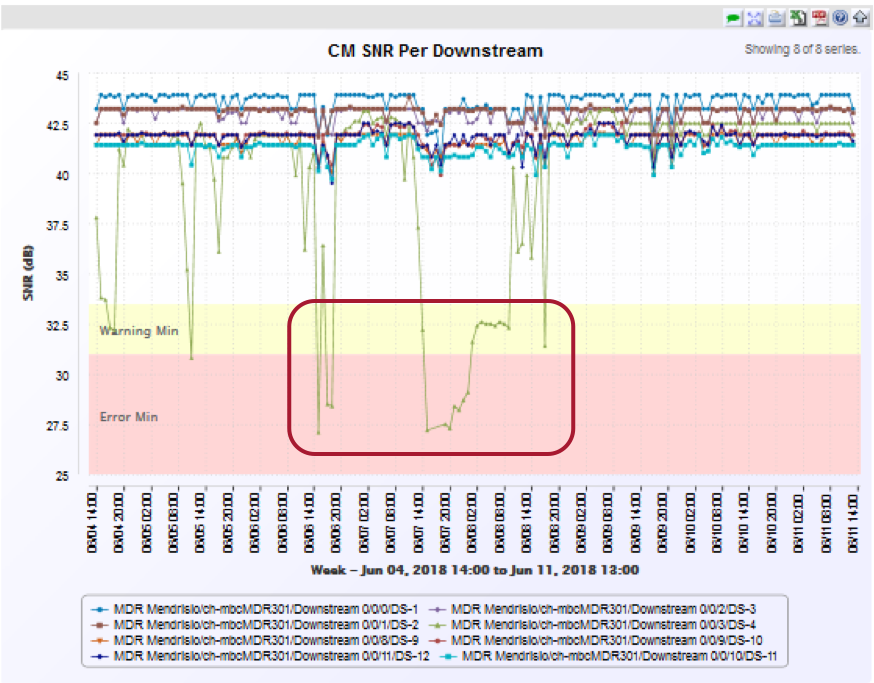
\includegraphics[width=1\linewidth]{thresholds}
    \end{center}
    \caption{Examples of graphs used by the \acrshort{hfc} support team to diagnose problems. Here for the downstream sound to noise ratio (allowed us to detect a service degradation)}.
    \label{thresholds}
\end{figure}

\subsection{Complex Models}
Some more complex models could be combined with an improved dataset. The \acrshort{poc} didn't contain any trial at deep learning given the engineering overhead as well as the results obtained with simpler model to support our goal.

\vspace{\baselineskip} 
All the tradeoffs related to our aim of building a \acrshort{poc} have been discussed and can obviously drive the development of a production ready tool.








